\documentclass[paper=a4,fontsize=10pt]{jlreq}
\usepackage{amsmath,amsfonts,array,ascmac,amssymb} %数学に必要なパッケージ
\usepackage{tikz} %グラフ描画に必要なパッケージ
\usepackage{TeachersGuide} %学習指導案パッケージ
\usepackage{multirow,tcolorbox} %表縦結合パッケージ
\usepackage{tcolorbox} %tcolorbox用のパッケージ
    \tcbuselibrary{raster,skins,breakable,theorems} %tcolorbox用のパッケージ
    \usetikzlibrary{calc} %グラフ描画に必要なパッケージ
\begin{document}
\showTitle{11月11日 1校時}{3年A組}{数学III}{数学III 数研出版}{溝口洸熙}
%\showTitle{授業日}{授業クラス}{授業科目}{仕様教科書}{指導教員}
\unitTitle{回転体の体積}
%\unitTitle{単元名}
\begin{UnitGoals} %単元の目標
    \begin{itemize}
        \item 目標1
        \item 目標2
    \end{itemize}
\end{UnitGoals}
\begin{UnitView} %単元観
    単元観を書く.\verb|\par|で改行字下げする.
\end{UnitView}
\begin{EvaluationCriterion} %評価規準
    \begin{enumerate}
        \enumiA %{fbox内に"A"と数字を記入する}
        \item 知識があるといいね
        \item 技能があるといいね
    \end{enumerate} &
    \begin{enumerate}
        \enumiB %{fbox内に"B"と数字を記入する}
        \item 思考があるといいね
        \item 判断があるといいね
        \item 表現があるといいね
    \end{enumerate} &
    \begin{enumerate}
        \enumiC %{fbox内に"C"と数字を記入する}
        \item 主体的に学習に取り組む態度があるといいね
    \end{enumerate}\\
    \hline
\end{EvaluationCriterion}
\begin{UnitPlan} %単元の授業計画・評価計画
    %n時間目 & n時間目の学習活動を書く. &  \fbox{評価規準と対応させる} & 評価方法を書く.
    第1時間目 & 1時間目の学習活動を書く.& \fbox{A1},\fbox{B2} & 観察・小テスト・自己評価\\
    \hline
    第2時間目 & 2時間目の学習活動を書く.& \fbox{B1},\fbox{B2} & 観察・ワークシート\\
    \hline
    第3時間目 & 3時間目の学習活動を書く.& \fbox{C1},\fbox{B1} & 観察・ワークシート・自己評価\\
\end{UnitPlan}
\begin{StudentFacts} %現在の生徒の実態を記入
    現在の生徒の実態を記入する.\verb|\par|で改行字下げする.
\end{StudentFacts}
\newpage
%----本時の計画----
\begin{ClassGoal} %到達目標
    \begin{itemize}
        \item 本時の到達目標その1.
        \item 本時の到達目標その2.
    \end{itemize}
\end{ClassGoal}
\begin{ClassPoint} %本時のポイント
    本時のポイントを書く.\verb|\par|で改行字下げする.
\end{ClassPoint}
\begin{TeachingProcedures} %本時の展開
    % 段階 & 学習活動 & 指導上の留意点 & 評価の観点
    % tpacol環境 & tpbcol環境 & tpccol環境 & tpdcol環境
    % 各環境はminipageを定義している.minipageの横幅情報は環境に含まれている.
    \begin{tpacol}
        \begin{center}
            導入
        \end{center}
    \end{tpacol}&
    \begin{tpbcol}
        この指導計画表は,何も意味がありません.ただ,できることを羅列しているだけです.\\
        \dotfill\\
        \verb|\dotfill\\|で,点線を挿入できる.
    \end{tpbcol}& &
    \\
    & \begin{tpbcol}
        \begin{framed}
            \noindent\textbf{復習問題1}\par
            曲線\(y=\sqrt{x}\)と\(x\)軸,及び2直線\(x=1\textrm{,}x=2\)で囲まれた部分の面積を求めよ.
        \end{framed}
        \begin{framed}
            \begin{minipage}[c]{0.4\linewidth}
                \noindent\textbf{解答}(期待する解答)
                \begin{equation*}
                    \begin{aligned}
                        S & =\int_{1}^{2}\sqrt{x}\quad dx                      \\
                          & = \left[\dfrac{2}{3}x^{\frac{3}{2}}\right]^{2}_{1} \\
                          & = \dfrac{2}{3}\cdot 2^{\frac{3}{2}}-\dfrac{2}{3}   \\
                          & =\dfrac{2}{3}\left(2\sqrt{2}-1\right)
                    \end{aligned}
                \end{equation*}
            \end{minipage}
            \begin{minipage}[c]{0.56\linewidth}
                \centering
                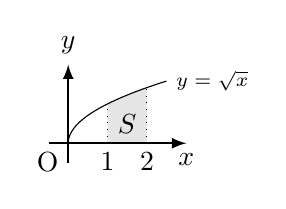
\begin{tikzpicture}[samples=300,scale=0.5]
                    \fill[fill=gray!20] plot[domain=1:2](\x, {sqrt(\x)})--(2,0)--(1,0)--cycle;
                    \draw[-latex,thick](-0.5,0)--(3,0)node[below]{\(x\)};
                    \draw[-latex,thick](0,-0.5)--(0,2)node[above]{\(y\)};
                    \node[below left] at(0,0){O};
                    \draw[domain=0:2.5] plot(\x, {sqrt(\x)})node[right]{\scriptsize \(y=\sqrt{x}\)};
                    \node at ($(2,0)!0.5!(1,1)$){\(S\)};
                    \draw[dotted](1,0)node[below]{1}--(1,1);
                    \draw[dotted](2,0)node[below]{2}--(2,{sqrt(2)});
                \end{tikzpicture}
            \end{minipage}
        \end{framed}
    \end{tpbcol} &
    \begin{tpccol}
        \begin{framed}
            \begin{verbatim}
\begin{framed}
    で,囲いができる.
\end{framed}
            \end{verbatim}
        \end{framed}
        \begin{tcolorbox}[title=tcolorbox]
            tcolorbox の設置も可能.
        \end{tcolorbox}
    \end{tpccol} &
    \begin{tpdcol}
    \end{tpdcol}\\
    \hline
    \begin{tpacol}
        \begin{center}
            展開
        \end{center}
    \end{tpacol}&
    \begin{tpbcol}
        \textbf{数式の表現}\\
        \verb|align,equation|で,数式に番号を振ったり,\(=\)で揃えたり.
        \begin{verbatim}
\begin{equation}
    \begin{aligned}
        V & = \int_{1}^{2} S(x) dx\\
        & = \pi\int_{1}^{2} 
            \big\{\sqrt{x}\big\}^2 dx = \pi
    \end{aligned}
\end{equation}
        \end{verbatim}
        \begin{equation}
            \begin{aligned}
                V & = \int_{1}^{2} S(x) dx                            \\
                  & = \pi\int_{1}^{2} \big\{\sqrt{x}\big\}^2 dx = \pi
            \end{aligned}
        \end{equation}
    \end{tpbcol} &
    \begin{tpccol}
        \textbf{頑張ったら回転体も描ける.}
        \begin{center}
            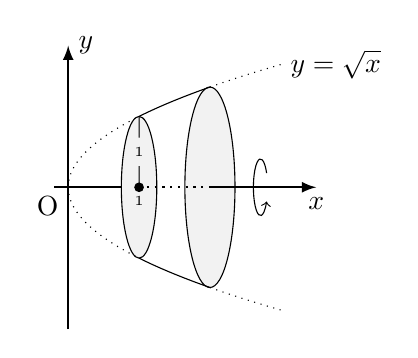
\begin{tikzpicture}[samples=300,scale=0.9]
                \def\Fx{plot(\x,{sqrt(\x)})};
                \def\dFx{plot(\x,{-1*sqrt(\x)})};
                \filldraw[draw=black,fill=gray!10](2,0)ellipse({sqrt(2)/4} and {sqrt(2)});
                \filldraw[draw=black,fill=gray!10](1,0)ellipse({sqrt(1)/4} and {sqrt(1)});
                \draw[domain=1:2] \Fx \dFx;
                \draw[domain=2:3,dotted] \Fx node[right]{\(y=\sqrt{x}\)} \dFx;
                \draw[domain=0:1,dotted] \Fx \dFx;
                \draw[thick](-0.2,0)--(0.75,0);
                \draw[thick,dotted](1,0)--(2,0);
                \draw[-latex,thick](2,0)--(3.5,0)node[below]{\(x\)};
                \draw[-latex,thick](0,-2)--(0,2)node[right]{\(y\)};
                \node[below left] at (0,0){O};
                \draw[->](2.8,0.2)arc[start angle=30, end angle=330, x radius=0.1, y radius=0.4];
                \node at (1,1/2)(r){\tiny 1};
                \draw[thin,fill=black](1,0)circle[radius=0.06]node[below]{\tiny 1}--(r)--(1,1);
            \end{tikzpicture}
            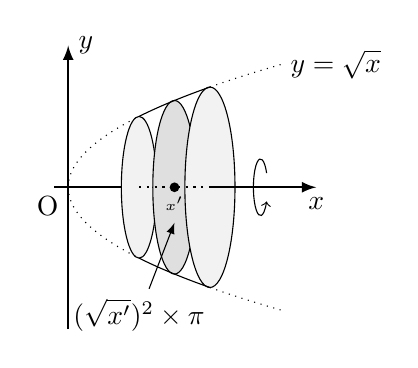
\begin{tikzpicture}[samples=300,scale=0.9]
                \def\Fx{plot(\x,{sqrt(\x)})};
                \def\dFx{plot(\x,{-1*sqrt(\x)})};
                \filldraw[draw=black,fill=gray!10](1,0)ellipse({sqrt(1)/4} and {sqrt(1)});
                \filldraw[draw=black,fill=gray!25](1.5,0)ellipse({sqrt(1.5)/4} and {sqrt(1.5)});
                \filldraw[draw=black,fill=gray!10](2,0)ellipse({sqrt(2)/4} and {sqrt(2)});
                \draw[domain=1:2] \Fx \dFx;
                \draw[domain=2:3,dotted] \Fx node[right]{\(y=\sqrt{x}\)} \dFx;
                \draw[domain=0:1,dotted] \Fx \dFx;
                \draw[thick](-0.2,0)--(0.75,0);
                \draw[thick,dotted](1,0)--(2,0);
                \draw[-latex,thick](2,0)--(3.5,0)node[below]{\(x\)};
                \draw[-latex,thick](0,-2)--(0,2)node[right]{\(y\)};
                \node[below left] at (0,0){O};
                \draw[->](2.8,0.2)arc[start angle=30, end angle=330, x radius=0.1, y radius=0.4];
                \draw[fill=black](1.5,0)circle[radius=0.06]node[below]{\tiny \(x'\)};
                \node at (1,-1.8)(s) {\((\sqrt{x'})^2\times \pi\)};
                \draw[-latex](s)--(1.5,-0.5);
            \end{tikzpicture} \\
        \end{center}
    \end{tpccol} &
    \begin{tpdcol}
    \end{tpdcol} \\
    &
    \begin{tpbcol}
        \textbf{一般化}\par
        \indent 一般的に,曲線\(y=f(x)\)と\(x\)軸,及び2直線\(x=a\textrm{,}x=b (a<b)\)で囲まれた部分を,\(x\)軸の周りに1回転させてできる立体の体積を\(V\)とすると,以下の公式が得られる.
        \begin{equation}
            \begin{aligned}
                V = \pi\int_{a}^{b}\big\{f(x)\big\}^2dx = \pi\int_{a}^{b}y^2dx
            \end{aligned}
        \end{equation}
        \begin{flushright}
            \((a<b)\)
        \end{flushright}
    \end{tpbcol} &
    \multicolumn{2}{c|}{%
        \begin{minipage}[t]{0.45\linewidth}
            \begin{framed}
                列を跨いで,いろいろできる.\\
                \textbf{オイラーの公式とオイラーの等式}
                \begin{equation}
                    \begin{aligned}
                        e^{i\theta} & = \cos\theta + i \sin\theta \\
                        e^{i\pi}    & = -1
                    \end{aligned}
                \end{equation}
            \end{framed}
        \end{minipage}
    }
    \\ & & 列を跨ぐために,\verb|\multicolumn|を利用する. & \\
    \begin{tpacol}
    \end{tpacol} &
    \multicolumn{2}{c|}{%
        \begin{minipage}{0.65\linewidth}
            \vspace{2em}
            \begin{framed}
                \textbf{微分の定義}
                \[ f’ (x) = \dfrac{d}{dx}f(x) = \lim_{h \to 0} \frac{f(x+h)– f(x)}{h} \]
            \end{framed}
        \end{minipage}
    } &
    \begin{tpdcol}
        \[{}_n\mathrm{C}_r=\dfrac{n!}{r!(n-r)!}\]
    \end{tpdcol}\\
\end{TeachingProcedures}
\end{document}